\subsection{随机性与非零模解析层的补充消融}
\label{sec:review-ablation}
为区分随机频率与解析外边界层的作用，我们预先固定两档配置
$(m,K,q,\Delta t^{-1})=(37,72,66,128)$、$(41,80,76,152)$，
将配对频率中的随机偏移 $\xi_j\sim U[0.2,0.8]$ 与确定性中点
$\xi_j=0.5$ 交叉比较，并分别保留或移除非零模的六个解析层函数。
随机组使用原先注册的五个种子（7331、7687、8011、8353、9041）；
每个确定性配置仅有一个独立轨迹，不将未使用的种子视为重复实验。
平均模始终保留相同的24个基函数与六个层函数、同一组积分点及时间步长。
适配器验证确认四组的平均模离散数组与隐式算子逐位一致。

第三版修订新增16条CPU $T=72$ 轨迹（14条消融及2条原配置复算控制），
复用并重新评分10条已冻结的随机加层GPU轨迹。
所有轨迹均在19个固定时刻、三个独立网格、两套细化FD参考上评价
全域与 $r\leq2.5$ 区域的速度和涡量；四项误差均须小于等于0.5\%。
表~\ref{tab:review-ablation} 报告每组跨种子、时刻、网格和参考的最坏相对误差。
16条CPU计算均完成，未出现数值运行失败；12条无层轨迹均为精度不达标。
两个CPU复算控制相对于归档GPU解的最坏场差异小于 $2.0\times10^{-10}$。

\begin{table}[htbp]
\centering\small
\caption{补充CPU精度消融。误差单位为\%；通过数不包含两条单列复算控制。
每行中的随机组为五个种子的最坏值，确定性组为一个配置。两条随机有层CPU复算相对归档GPU控制的四项场范数偏差均小于 $2.0\times10^{-10}$；该界不覆盖其它消融分支。}
\label{tab:review-ablation}
\begin{tabular}{lrrrrrr}
\hline
配置 & 秩 & $e_u$ & $e_\omega$ & $e_{u,\mathrm{near}}$ & $e_{\omega,\mathrm{near}}$ & 通过 \\
\hline
中, 随机+层 & 39 & 0.0294 & 0.4096 & 0.0251 & 0.2100 & 5/5 \\
中, 定点+层 & 39 & 0.0293 & 0.4092 & 0.0249 & 0.2097 & 1/1 \\
中, 随机无层 & 34 & 19.4054 & 73.8980 & 26.4854 & 48.6306 & 0/5 \\
中, 定点无层 & 34 & 19.3644 & 73.7836 & 26.4397 & 48.5825 & 0/1 \\
高, 随机+层 & 40 & 0.0182 & 0.3319 & 0.0148 & 0.1799 & 5/5 \\
高, 定点+层 & 40 & 0.0181 & 0.3312 & 0.0147 & 0.1794 & 1/1 \\
高, 随机无层 & 35 & 18.7540 & 72.0115 & 25.7262 & 47.7640 & 0/5 \\
高, 定点无层 & 35 & 18.7060 & 71.8705 & 25.6678 & 47.6945 & 0/1 \\
\hline
\end{tabular}
\end{table}

确定性中点加层的两档配置均通过门槛，其误差与随机加层组相当，
因此这些数据不支持将随机性视为当前精度优势的必要来源。
在固定原始 $m$ 与SVD截断阈值的设计下，去除非零模层函数使保留秩由
39/40降为34/35，并导致很大的速度与涡量误差；平均模的保留秩始终为30。
这表明现有紧凑配置高度依赖解析外边界层富集，但不能把其作用与增加的有效维数完全分开：
此处并非等秩层函数消融，也没有遍历所有确定性频率设计。
两档确定性无层配置的四项最坏误差均出现在 $T=72$；
其早期 $t\leq16$ 的最大涡量误差为2.820\%和2.592\%，随后分别增至73.784\%和71.871\%。
因此，表中的大误差并非由起始时刻近零参考场单独造成，但这些数据尚不能确定误差放大的具体动力学机制。
随后仅作构造检查：保持频率带宽62、积分点和截断阈值不变，
将无层确定性基的原始 $m$ 依次增加至41、45、49、53、57、61，
两档的保留秩均为35、35、36、36、36、36，未恢复至39或40。
因此没有追加声称等秩的 $T=72$ 对照，也没有为通过门槛而继续调整带宽或截断阈值。
并行CPU耗时只作为运行诊断，不构成新的隔离计时或GPU加速证据，
原78条GPU资格实验的边界保持不变。

\paragraph{富集空间对照能识别与不能识别的因素。}
Legendre35 和 Legendre36 控制同样包含式~\eqref{eq:layer-features}中的六个解析层函数。因此，本实验并没有证明“无富集的 Legendre 成功而无富集的三角空间失败”。同一分辨率下两族使用同一套预设径向求积；选择 Legendre 试验基不会自动把它替换为该基族专有的 Gauss--Lobatto 网格。多项式插值节点的端点聚束因而不是本对照中实测改变的解释变量。无富集且匹配保留秩的多项式控制仍需单独实验。

层函数按 $e^{-\gamma(L-s)}$ 衰减，集中在\emph{外边界} $s=L$，而不是圆柱内壁 $s=0$。此外，当前远场齐次算子采用 $\chi=16z^2(1-z)$ 和式~\eqref{eq:boundary-transform}中的修正；其无滑移条件并不强迫内壁曲率为零。以撇号表示 $z$ 导数，有 $(\mathcal Bq)''(0)=32q(0)-[(\chi q)'']_{z=1}$，通常非零。因此，仅凭删除这些层函数不能建立“内壁曲率自由度丢失导致分离角改变”的因果链。末态大误差表明当前结果对试验空间和保留维数共同敏感；固定中点设计与五个抽样种子的最坏误差相当或稍好，也不是随机化永远无益的定理。


\paragraph{保存探针对累计相位漂移的证据。}
进一步分析间隔 $0.125$ 的既有577次观测，不新增轨迹积分，也不平移物理评分时刻。主窗口为 $24\leq t\leq72$：去除最小二乘线性趋势后，线性插值上穿零点，再将过零时刻对事件序号作仿射拟合，以斜率倒数估计频率。保留 $x=1.5,2.5,3.5$、$y=0$ 三点的速度和涡量，另以36、48为窗口起点、仅去均值以及两套细FD参考检查敏感性。这些有限窗口估计是描述性诊断，不是置信区间或无限外域Strouhal数验证。

\begin{table}[htbp]
\centering\small
\caption{既有固定中点频率轨迹在 $[24,72]$、$(2.5,0)$ 处的涡量诊断，参考为时间细化FD。每个拟合含8个上穿零点，即7个完整间隔；参考频率为 $0.17534308$。频偏单位为百分比，延迟为匹配参考过零时刻 $t=66.797754$ 时候选减参考的时间差。}
\label{tab:review-phase-probes}
\begin{tabular}{llrrrr}
\toprule
分辨率 & 非零模层函数 & 秩 & 频率 & 频偏(\%) & 延迟\\
\midrule
中档 & 保留 & 39 & 0.17534574 & $+0.00152$ & $-0.00101$\\
中档 & 删除 & 34 & 0.16799056 & $-4.19322$ & $+1.75259$\\
高档 & 保留 & 40 & 0.17534385 & $+0.00044$ & $-0.00020$\\
高档 & 删除 & 35 & 0.16837253 & $-3.97538$ & $+1.67221$\\
\bottomrule
\end{tabular}
\end{table}

五个随机种子与中点控制的全部无层配置，在主窗口六条探针信号上的频偏范围为 $-4.27\%$ 至 $-3.35\%$；纳入两参考、三窗口及两种去趋势方式后，范围扩展为 $-5.20\%$ 至 $-1.88\%$。图~\ref{fig:review-phase-probes}中逐渐增大的过零延迟，支持累计相位漂移是长期失配的一部分。两条中点无层配置的 $2\pi(f-f_{\rm ref})48$ 分别约为 $-2.22$、$-2.10$ 弧度，但这只是拟合频率差的累计估计，不是实测全场相位修正。数据不能将约 $70\%$ 的场误差全部归于相位。删除的是局限于\emph{外边界}的富集函数，保留秩也同时变化，且没有测量内壁分离角，因此尚未建立“内壁欠分辨导致频偏”的因果链。

\begin{figure}[htbp]
\centering
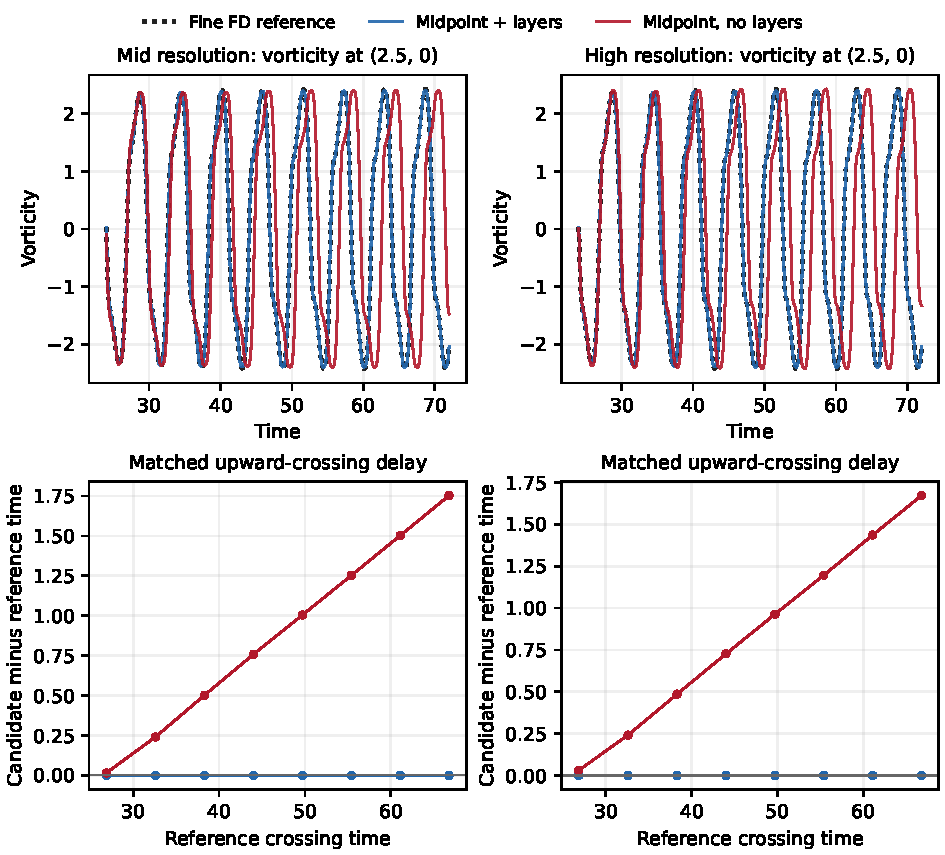
\includegraphics[width=\linewidth]{figures/review_phase_probes.pdf}
\caption{固定中点频率消融的原始时刻涡量信号及累计过零延迟。先将候选第一个相关过零事件与最近的初始参考事件配对，此后保持事件序号。下排仅在事件检测时去除线性趋势，没有平移任何轨迹或场误差评分。}
\label{fig:review-phase-probes}
\end{figure}

